\documentclass[12pt, conference, letterpaper]{IEEEtran}
\usepackage{tikz}
\usepackage{cuted}
\usetikzlibrary{automata,positioning}

% *** CITATION PACKAGES ***
%
\ifCLASSOPTIONcompsoc
  % IEEE Computer Society needs nocompress option
  % requires cite.sty v4.0 or later (November 2003)
  \usepackage[nocompress]{cite}
\else
  % normal IEEE
  \usepackage{cite}
  \usepackage{graphicx}
  \usepackage{amsmath}
\usepackage[utf8]{inputenc}
\usepackage{amsmath, amssymb, latexsym}

\usepackage[left=2cm,right=2cm,top=2cm,bottom=2cm]{geometry}
\usepackage{tikz}
\usepackage{tikz-cd}
\usetikzlibrary{decorations.pathreplacing}
\usetikzlibrary{fadings}

\usetikzlibrary{quotes,arrows.meta}
\tikzset{
  annotated cuboid/.pic={
    \tikzset{%
      every edge quotes/.append style={midway, auto},
      /cuboid/.cd,
      #1
    }
    \draw [every edge/.append style={pic actions, densely dashed, opacity=.5}, pic actions]
    (0,0,0) coordinate (o) -- ++(-\cubescale*\cubex,0,0) coordinate (a) -- ++(0,-\cubescale*\cubey,0) coordinate (b) edge coordinate [pos=1] (g) ++(0,0,-\cubescale*\cubez)  -- ++(\cubescale*\cubex,0,0) coordinate (c) -- cycle
    (o) -- ++(0,0,-\cubescale*\cubez) coordinate (d) -- ++(0,-\cubescale*\cubey,0) coordinate (e) edge (g) -- (c) -- cycle
    (o) -- (a) -- ++(0,0,-\cubescale*\cubez) coordinate (f) edge (g) -- (d) -- cycle;
    \path [every edge/.append style={pic actions, |-|}]
    (b) +(0,-3.9pt) coordinate (b1) edge ["\cubex "'] (b1 -| c)
    (b) +(-3.9pt,0) coordinate (b2) edge ["\cubey "] (b2 |- a)
    (c) +(3.5pt,-3.5pt) coordinate (c2) edge ["\cubez "'] ([xshift=3.5pt,yshift=-3.5pt]e)
    ;
  },
  /cuboid/.search also={/tikz},
  /cuboid/.cd,
  width/.store in=\cubex,
  height/.store in=\cubey,
  depth/.store in=\cubez,
  scale/.store in=\cubescale,
  width=10,
  height=10,
  depth=10,
  scale=.1,
}

\tikzset{
  annotated rectangle/.pic={
    \tikzset{%
      every edge quotes/.append style={midway, auto},
      /cuboid/.cd,
      #1
    }
    \draw [every edge/.append style={pic actions, densely dashed, opacity=.5}, pic actions]
    (0,0,0) coordinate (o) -- ++(-\cubescale*\cubex,0,0) coordinate (a) -- ++(0,-\cubescale*\cubey,0) coordinate (b) edge coordinate [pos=1] (g) ++(0,0,-\cubescale*\cubez)  -- ++(\cubescale*\cubex,0,0) coordinate (c) -- cycle
    (o) -- ++(0,0,-\cubescale*\cubez) coordinate (d) -- ++(0,-\cubescale*\cubey,0) coordinate (e) edge (g) -- (c) -- cycle
    (o) -- (a) -- ++(0,0,-\cubescale*\cubez) coordinate (f) edge (g) -- (d) -- cycle;
    \path [every edge/.append style={pic actions, |-|}]
   
    (b) +(-3.9pt,0) coordinate (b2) edge ["\cubey "] (b2 |- a)
    ([xshift=3.5pt,yshift=-3.5pt]e)
    ;
  },
  /cuboid/.search also={/tikz},
  /cuboid/.cd,
  width/.store in=\cubex,
  height/.store in=\cubey,
  depth/.store in=\cubez,
  scale/.store in=\cubescale,
  width=10,
  height=10,
  depth=10,
  scale=.1,
}
%
\makeatletter
\setlength{\@fptop}{0pt}
\makeatother
%
\fi



% cite.sty was written by Donald Arseneau
% V1.6 and later of IEEEtran pre-defines the format of the cite.sty package
% \cite{} output to follow that of the IEEE. Loading the cite package will
% result in citation numbers being automatically sorted and properly
% "compressed/ranged". e.g., [1], [9], [2], [7], [5], [6] without using
% cite.sty will become [1], [2], [5]--[7], [9] using cite.sty. cite.sty's
% \cite will automatically add leading space, if needed. Use cite.sty's
% noadjust option (cite.sty V3.8 and later) if you want to turn this off
% such as if a citation ever needs to be enclosed in parenthesis.
% cite.sty is already installed on most LaTeX systems. Be sure and use
% version 5.0 (2009-03-20) and later if using hyperref.sty.
% The latest version can be obtained at:
% http://www.ctan.org/pkg/cite
% The documentation is contained in the cite.sty file itself.
%
% Note that some packages require special options to format as the Computer
% Society requires. In particular, Computer Society  papers do not use
% compressed citation ranges as is done in typical IEEE papers
% (e.g., [1]-[4]). Instead, they list every citation separately in order
% (e.g., [1], [2], [3], [4]). To get the latter we need to load the cite
% package with the nocompress option which is supported by cite.sty v4.0
% and later.





% *** GRAPHICS RELATED PACKAGES ***
%
\ifCLASSINFOpdf
  % \usepackage[pdftex]{graphicx}
  % declare the path(s) where your graphic files are
  % \graphicspath{{../pdf/}{../jpeg/}}
  % and their extensions so you won't have to specify these with
  % every instance of \includegraphics
  % \DeclareGraphicsExtensions{.pdf,.jpeg,.png}
\else
  % or other class option (dvipsone, dvipdf, if not using dvips). graphicx
  % will default to the driver specified in the system graphics.cfg if no
  % driver is specified.
 % \usepackage[dvips]{graphicx}
  % declare the path(s) where your graphic files are
  % \graphicspath{{../eps/}}
  % and their extensions so you won't have to specify these with
  % every instance of \includegraphics
  % \DeclareGraphicsExtensions{.eps}
\fi
% graphicx was written by David Carlisle and Sebastian Rahtz. It is
% required if you want graphics, photos, etc. graphicx.sty is already
% installed on most LaTeX systems. The latest version and documentation
% can be obtained at: 
% http://www.ctan.org/pkg/graphicx
% Another good source of documentation is "Using Imported Graphics in
% LaTeX2e" by Keith Reckdahl which can be found at:
% http://www.ctan.org/pkg/epslatex
%
% latex, and pdflatex in dvi mode, support graphics in encapsulated
% postscript (.eps) format. pdflatex in pdf mode supports graphics
% in .pdf, .jpeg, .png and .mps (metapost) formats. Users should ensure
% that all non-photo figures use a vector format (.eps, .pdf, .mps) and
% not a bitmapped formats (.jpeg, .png). The IEEE frowns on bitmapped formats
% which can result in "jaggedy"/blurry rendering of lines and letters as
% well as large increases in file sizes.
%
% You can find documentation about the pdfTeX application at:
% http://www.tug.org/applications/pdftex



%\usepackage{epstopdf}

% *** MATH PACKAGES ***
%
\usepackage{amsthm,amsmath}
\newtheorem{mydef}{Definition}
% A popular package from the American Mathematical Society that provides
% many useful and powerful commands for dealing with mathematics.
%
% Note that the amsmath package sets \interdisplaylinepenalty to 10000
% thus preventing page breaks from occurring within multiline equations. Use:
%\interdisplaylinepenalty=2500
% after loading amsmath to restore such page breaks as IEEEtran.cls normally
% does. amsmath.sty is already installed on most LaTeX systems. The latest
% version and documentation can be obtained at:
% http://www.ctan.org/pkg/amsmath





% *** SPECIALIZED LIST PACKAGES ***
%
%\usepackage{algorithmic}
% algorithmic.sty was written by Peter Williams and Rogerio Brito.
% This package provides an algorithmic environment fo describing algorithms.
% You can use the algorithmic environment in-text or within a figure
% environment to provide for a floating algorithm. Do NOT use the algorithm
% floating environment provided by algorithm.sty (by the same authors) or
% algorithm2e.sty (by Christophe Fiorio) as the IEEE does not use dedicated
% algorithm float types and packages that provide these will not provide
% correct IEEE style captions. The latest version and documentation of
% algorithmic.sty can be obtained at:
% http://www.ctan.org/pkg/algorithms
% Also of interest may be the (relatively newer and more customizable)
% algorithmicx.sty package by Szasz Janos:
% http://www.ctan.org/pkg/algorithmicx




% *** ALIGNMENT PACKAGES ***
%
%\usepackage{array}
% Frank Mittelbach's and David Carlisle's array.sty patches and improves
% the standard LaTeX2e array and tabular environments to provide better
% appearance and additional user controls. As the default LaTeX2e table
% generation code is lacking to the point of almost being broken with
% respect to the quality of the end results, all users are strongly
% advised to use an enhanced (at the very least that provided by array.sty)
% set of table tools. array.sty is already installed on most systems. The
% latest version and documentation can be obtained at:
% http://www.ctan.org/pkg/array


% IEEEtran contains the IEEEeqnarray family of commands that can be used to
% generate multiline equations as well as matrices, tables, etc., of high
% quality.




% *** SUBFIGURE PACKAGES ***
%\ifCLASSOPTIONcompsoc
%  \usepackage[caption=false,font=footnotesize,labelfont=sf,textfont=sf]{subfig}
%\else
%  \usepackage[caption=false,font=footnotesize]{subfig}
%\fi
% subfig.sty, written by Steven Douglas Cochran, is the modern replacement
% for subfigure.sty, the latter of which is no longer maintained and is
% incompatible with some LaTeX packages including fixltx2e. However,
% subfig.sty requires and automatically loads Axel Sommerfeldt's caption.sty
% which will override IEEEtran.cls' handling of captions and this will result
% in non-IEEE style figure/table captions. To prevent this problem, be sure
% and invoke subfig.sty's "caption=false" package option (available since
% subfig.sty version 1.3, 2005/06/28) as this is will preserve IEEEtran.cls
% handling of captions.
% Note that the Computer Society format requires a sans serif font rather
% than the serif font used in traditional IEEE formatting and thus the need
% to invoke different subfig.sty package options depending on whether
% compsoc mode has been enabled.
%
% The latest version and documentation of subfig.sty can be obtained at:
% http://www.ctan.org/pkg/subfig




% *** FLOAT PACKAGES ***
%
%\usepackage{fixltx2e}
% fixltx2e, the successor to the earlier fix2col.sty, was written by
% Frank Mittelbach and David Carlisle. This package corrects a few problems
% in the LaTeX2e kernel, the most notable of which is that in current
% LaTeX2e releases, the ordering of single and double column floats is not
% guaranteed to be preserved. Thus, an unpatched LaTeX2e can allow a
% single column figure to be placed prior to an earlier double column
% figure.
% Be aware that LaTeX2e kernels dated 2015 and later have fixltx2e.sty's
% corrections already built into the system in which case a warning will
% be issued if an attempt is made to load fixltx2e.sty as it is no longer
% needed.
% The latest version and documentation can be found at:
% http://www.ctan.org/pkg/fixltx2e


%\usepackage{stfloats}
% stfloats.sty was written by Sigitas Tolusis. This package gives LaTeX2e
% the ability to do double column floats at the bottom of the page as well
% as the top. (e.g., "\begin{figure*}[!b]" is not normally possible in
% LaTeX2e). It also provides a command:
%\fnbelowfloat
% to enable the placement of footnotes below bottom floats (the standard
% LaTeX2e kernel puts them above bottom floats). This is an invasive package
% which rewrites many portions of the LaTeX2e float routines. It may not work
% with other packages that modify the LaTeX2e float routines. The latest
% version and documentation can be obtained at:
% http://www.ctan.org/pkg/stfloats
% Do not use the stfloats baselinefloat ability as the IEEE does not allow
% \baselineskip to stretch. Authors submitting work to the IEEE should note
% that the IEEE rarely uses double column equations and that authors should try
% to avoid such use. Do not be tempted to use the cuted.sty or midfloat.sty
% packages (also by Sigitas Tolusis) as the IEEE does not format its papers in
% such ways.
% Do not attempt to use stfloats with fixltx2e as they are incompatible.
% Instead, use Morten Hogholm'a dblfloatfix which combines the features
% of both fixltx2e and stfloats:
%
% \usepackage{dblfloatfix}
% The latest version can be found at:
% http://www.ctan.org/pkg/dblfloatfix




% *** PDF, URL AND HYPERLINK PACKAGES ***
%
%\usepackage{url}
% url.sty was written by Donald Arseneau. It provides better support for
% handling and breaking URLs. url.sty is already installed on most LaTeX
% systems. The latest version and documentation can be obtained at:
% http://www.ctan.org/pkg/url
% Basically, \url{my_url_here}.




% *** Do not adjust lengths that control margins, column widths, etc. ***
% *** Do not use packages that alter fonts (such as pslatex).         ***
% There should be no need to do such things with IEEEtran.cls V1.6 and later.
% (Unless specifically asked to do so by the journal or conference you plan
% to submit to, of course. )


% correct bad hyphenation here
%\hyphenation{op-tical net-works semi-conduc-tor}




\begin{document}


\title{Adversarial Image Generation for Deep Learning Systems}


\author{\IEEEauthorblockN{Anonymous Bot
}
\IEEEauthorblockA{Department of 
Computer Science,
University of California, Davis\\
1 Shields Ave, Davis, CA 95616\\
}}







\maketitle
\begin{abstract}
Deep Neural Networks have become part of every day life and it is imperative that the robustness of these systems be ascertained using mathematical models. 
Classifiers can be made more robust by training with varying distributions. A way to do this is to create adversarial samples so as to regularize the neural network during training. In this work we combine some of the state of the art white box attacks to generate adversarial samples for Neural Networks as well as propose our own black box attack oblivious to the original Neural Network parameters. The results show that the white box attacks work for any network architecture while the black box attacks work infrequently as the network gets deeper.
\end{abstract}


\IEEEpeerreviewmaketitle



\section{Introduction}
Deep Neural Networks (DNNs) are considered the cutting edge technology to make decisions regarding image classification, voice recognition, advertising, bioinformatics, credit assessment, drug discovery and toxicology, etc. Accordingly, it is important to understand the threat model associated with Deep Neural Networks. Recent research \cite{1}, \cite{2} has shown that it is possible to generate adversarial examples in speech that can be interpreted by machines but not humans. Consequently, it is possible to control someone’s phone without the person's knowledge.\cite{8} This has also been expanded to images\cite{3}, where small perturbations in the image pixels was sufficient to fool a trained Neural Network. 
In this regard our contribution is to formulate, using methods of Computer Vision, a way to create adversarial images for trained Deep Neural Network. The motivation for this work comes from the fact that machines can classify captchas with almost human accuracy. Our goal is to create images that can be correctly classified by humans but not by a Deep Neural Networks. \newline

We begin by distorting the image in specific ways so as to increase the error rate of the targeted deep neural network. Initially we test our samples on a three layer Deep Neural Network to gain more intuition into the learning process and use the templates the Network learns at the end as a way to create additional adversarial samples. 
In our first attack approach, we train another neural network, called an Adversarial Transformative Network (ATN) \cite{13}, to generate distortions in the input image. Existing ATN implementations don't restrict the distortions to be within a user-defined neighborhood. Our work, on the other hand, modifies the behavior of an ATN to restrict it to a neighborhood. For our second attack approach, we extend our idea to break a Deep Convolutional Neural Network (CNN), where we don't use the parameters of the target Deep CNN.This attack is oblivious to the target CNN parameters like architecture and weights.

\section{Background}
In this section we summarize existing techniques for generating adversarial images and also explore their limitations. \newline \newline
\textbf{2.1 Adversarial Examples} \newline
\indent Szegedy et al. first introduced the term "adversarial examples" in 2014; that is, inputs with slight perturbations which trick modern neural network models into misclassifying data. \cite{4} This indicates that even cutting edge neural networks which perform excellently on the test set, utterly fail compared to humans, when the data is perturbed slightly. These adversarial examples are particularly robust, which means adversarial examples generated on one neural network can trick another neural network trained with completely different parameters. \cite{5} In certain datasets, including the ImageNet \cite{6} dataset, the adversarial examples were almost indistinguishable to the human eye. This clearly points out a security threat associated with machine learning models. \newline \newline

\begin{figure}[h]
\includegraphics[scale=0.45]{pictures/whitebox.png}
\caption{ Overview of three different types of attacks on DNNs.In the black box attack, the attacker can input an example and only observe the output(Query), while in the white box attack the attacker can also access the internal parameters of the DNN(Back Propagation). \cite{10}}
\end{figure} 

\noindent{{\bf 2.2 Types of Attacks:}\\
\indent Current adversarial attack  methods can be divided into several categories based on what information they have access to. In a white box attack, the attacker has access to the weights and the architecture of the target network. This can also include attacks which have access to the data which the target network was trained on. In a black box attack, the attacker only has access to the final output of the network. For an image classifier, this would be the predicted class of the image. Furthermore, some attacks seek to simply cause the image to be misclassified, while others seek to have the perturbed image classified as a specific class. An overview of these attacks is given in Figure 1. \cite{14} \newline

\noindent{{\bf 2.3 Linear explanation of Adversarial Examples and the Fast Gradient Sign Method}\\
\indent In 2015, Goodfellow et al. at Google Inc. hypothesized that the underlying cause of neural networks not being able to correctly classify adversarial examples is due to their inherent linearity. This essentially means that adversarial examples can be generated for simple linear models if its inputs have sufficient dimensionality. In many problems the input precision is limted. For instance, for an image using 8-bits per pixel, the model would discard all information below 1/255 of the dynamic range. Thus an input image \textbf{x} would be considered to be same as an adversarial input \textbf{x' = x + $\eta$} by the classifier. An example is shown in Figure 2. They also demonstrated a method of generating adversarial examples, the "fast gradient sign method". In this method adversarial perturbations can be quickly and easily generated by adding a small vector along the direction of increasing the cost. \cite{5} \newline

\begin{figure}[h]
\includegraphics[scale=0.35]{pictures/pandaimagenet.png}
\caption{ In 2015, Goodfellow et al. demonstrated adversarial example generation applied to GoogLeNet on ImageNet. This demonstrates the Fast Gradient Sign Method. Here .007 is the magnitude of the smallest bit of an 8-bit image encoding.\cite{5}}
\end{figure}
Although the FGSM method is fast and efficient, it has been shown in later works to be easily defended against. Despite this, FGSM gives the clearest intuition on generating adversarial examples, and has inspired most other techniques. Even our work derives from this method's idea of confining perturbations within a neighborhood. \newline \newline
\noindent{{\bf 2.4 JSMA}\\
\indent Jacobian-based Saliency Map Attack (JSMA) is an attack optimized under $L_0$ introduced by Papernot et al. Similar to FGSM, this method seeks to make small changes in the input image to produce a perturbed image. This method seeks to modify only certain features of the input and create a perturbed input which will be classified as a target class. The main innovation in this approach is the ability to find the important features in the input, which when modified, will lead to a target classification by the model. To do this, we can construct an adversarial saliency map.\cite{7} \cite{8} \newline

JSMA uses an adversarial saliency map, shown in Figure 3, which shows the best features to be perturbed in an input to generate the desired classification. This saliency map is constructed using the forward derivative of the target network. High values in the saliency map correspond to features that will increase the probability of the input being classified as a target class or decrease the probability of the input being classified as another classes.
\newline

After obtaining the saliency map, we can use it to perturb the given input. There are two new parameters to keep in mind here. First, $\theta$ defines the amount by which a feature is perturbed. Second, $\upsilon$ defines the maximum number of epochs that the algorithm can run for. Both of these parameters serve to minimize the distortion to the image and should be adjusted depending on the specific problem. \newline

JSMA searches for a pair of pixels which can be modified to increase the likelihood of the target class and reduce that of the other classes. This has been shown to be a drawback of this algorithm. When it comes to large images, such as $1000 X 1000 X 3$, it would be computationally expensive to search through all of the pairs of pixels.\cite{8}
\begin{figure}[h]
\includegraphics[scale=0.35]{pictures/saliencymap.png}
\caption{ Saliency map of a 28 x 28 image generated by JSMA. Those points with large absolute values have greatest effect on the classification of the image. \cite{9}}
\end{figure}  \newline

\noindent{{\bf 2.5 Carlini \& Wagner (C\&W) Attack }\\
\indent In 2016, Carlini and Wagner proposed a strong white box attack. Being a white box attack they take advantage of the internal parameters of a targeted DNN and designed adversarial attacks as an optimization problem. \cite{8} They use the Euclidean distance, which is the $L_2$ norm, to assess the difference between adversarial and original examples.The new image is optimized by the Euclidian norm to be close to the original image. Given an image, the C\&W method generates a perturbed image which is classified as a target class. The perturbation is also optimized to have the highest probability of being classified as the target class. They also showed that their attack bypasses the ten different methods designed for detecting adversarial examples.\cite{11} However, the defence models proposed by Aleksander Madry et al. showed favorable results against the C\&W attack, as well as FGSM.\cite{10} \cite{12}


\section{White Box Adversarial Transformative Networks:}

\noindent{{\bf 3.1 Adversarial Transformative Networks}\\
\indent Adversarial Transformative Networks (ATNs) were proposed in 2017 by 
Baluja and Fischer in 2017 in their paper, Adversarial Transformative 
Networks: Learning to Generate Adversarial Examples. In contrast to 
other methods such as FGSM or JSMA that generate adversarial examples 
directly by computing gradients on the image pixels or solving an 
optimization problem on them, ATN is by itself a neural network that 
transforms an input into an adversarial example against a target network 
or a set of networks. ATNs can be targeted or untargeted and can also be 
trained in a black-box or a white-box manner. \cite{13}



We define the target neural network as y = f$_{w}$(x), with $w$ 
being the parameter matrix of the network $f$, and $x$ is the input. The output of 
$f$, $y$ is a vector representing the class probabilities for each label. 
The ATN is formally defined as $x' = g_{f,\theta} (x). \theta 
$ is the parameter matrix of the ATN and $x'$ is the adversarial 
transformation of $x$, such that $x'$ $\sim$ $x$, but argmax f$_{w}$(x) $\neq$ f$_{w}$(x').\cite{13} \newline


\noindent{{\bf 3.2 Cost Function}\\
\indent The parameters $\theta $ are obtained by solving an optimization on the 
cost function defined as follows:



\begin{figure}[h!]
    
    \label{fig:cclogo}
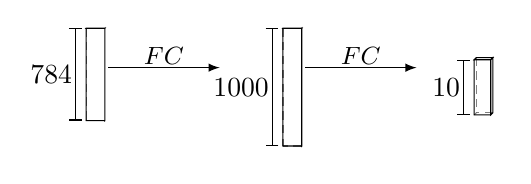
\begin{tikzpicture}[inner sep=1pt, >=latex, 
   label/.style={auto, inner sep=1pt, circle}
   ]
   
   \path (-10,-0.5) node (A) {$$}
   (-8.5,-0.5) node (B) {$$};
   \path (-7.5,-0.5) node (C) {$$}
   (-6,-0.5) node (D) {$$};
   
   \draw[->] (A) -- node[anchor=south] {\small $FC$} (B);
   
   \draw[->] (C) -- node[anchor=south, align=center] {\small $FC$} (D);
   
  \pic at (-10,0) {annotated rectangle={width=160, height=784, depth=1, scale = 0.0015}};
  \pic at (-7.5,0) {annotated rectangle={width=160, height=1000, depth=1, scale = 0.0015}};
  \pic at (-5.1,-0.4) {annotated rectangle={width=3, height=10, depth=1, scale = 0.07}};
  
\end{tikzpicture}
\caption{Architecture of target ANN}
\end{figure}


\indent $$\sum\limits_{x_{i}\in X}\beta L_{x}(g_{f, \theta}
(x_{i}), x_{i}) + L_{y}(f(g_{f, \theta}
(x_{i})),f(x_{i}))$$


$L_{x}$ is a measure of the difference between the generated 
adversarial example and the original input. $L_{y }$is a measure of 
the difference between the output generated by $f$ on an adversarial 
example and a particular target output for a targeted attack. For an 
untargeted attack, $L_{y}$ can be taken as a measure of likelihood 
between the output generated by $f$ on an adversarial example to the 
output generated by $f$ on the corresponding original input. In both 
cases, the goal is to identify values for $\theta $ that minimize both 
$L_{x}$ and $L_{y}$, and thus, the entire cost function. $\beta 
$ is tuning parameter to balance out the two terms.



For untargeted attacks, $L_{x}$ and $L_{y}$ can both be 
represented by straightforward $L_{1}$ or $L_{2}$ costs. For 
targeted attacks, $L_{x}$ can be a simple straightforward $L_{1}$ 
or $L_{2}$ loss, but $L_{y}$ would have to be modified to bias the 
learning towards the targeted task. To do this, the definition of $L{
_y}$ is modified to include a re-ranking function. Thus we could have a 
definition such as,
$$ L_{y} = L_{y}(f_{w}(g_{\theta}
(x_{i})),r(f_{w}(x), t)  $$
Here, $r$ is the re-ranking function, and $t$ is the target class that we're 
trying to make the classifier output. The choice of $r()$ can be used to 
tune the rate of training. For instance, $r$ can return a vector 
containing just a one-hot encoding, such that only the value 
corresponding to the target class is 1, with all others being 0. This 
approach however, does not make use of the probabilities that are 
computed by $f$ to drive the biasing. Hence, a better re-ranking function 
would be,

$$ r(f_{w}(x),t) = norm(\alpha *max(f_{w}(x))); k = t,$$
$$ r(f_{w}(x),t) = norm(f_{w}(x)); otherwise $$

\begin{figure}[h]
   
   \label{fig:cclogo}
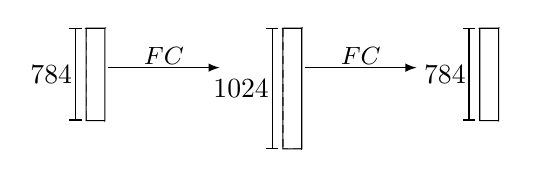
\begin{tikzpicture}[inner sep=1pt, >=latex, 
   label/.style={auto, inner sep=1pt, circle}
   ]
   
   \path (-10,-0.5) node (A) {$$}
   (-8.5,-0.5) node (B) {$$};
   \path (-7.5,-0.5) node (C) {$$}
   (-6,-0.5) node (D) {$$};
   
   \draw[->] (A) -- node[anchor=south] {\small $FC$} (B);
   
   \draw[->] (C) -- node[anchor=south, align=center] {\small $FC$} (D);
   
  \pic at (-10,0) {annotated rectangle={width=160, height=784, depth=1, scale = 0.0015}};
  \pic at (-7.5,0) {annotated rectangle={width=160, height=1024, depth=1, scale = 0.0015}};
  \pic at (-5,0) {annotated rectangle={width=160, height=784, depth=1, scale = 0.0015}};
  
\end{tikzpicture}
\caption{Architecture of ATN}
\end{figure}

Where, $norm$ is a standard normalization function, $k$ represents the 
possible output classes and $max()$ returns the max value of its input 
vector. $\alpha $ $>$ 1, is an additional parameter that ensures that 
the reranked output points only towards one particular class.\cite{13}
For example, if an output of a target neural network outputting three labels was (0.1, 0.2, 0.3), then after re-ranking, it would become (0.6, 0.2, 0.3), before normalizing. Here, the target label is the first label and the $\alpha$ parameter's value is 2. This vector gives more weight to the target label than a one-hot vector, which would just be (1, 0, 0) \newline


\noindent{{\bf 3.3 Our Approach}\\
\indent Once the parameters are obtained, the ATN can be used to generate a 
perturbation to each node of the input, thereby giving a new adversarial 
input. One point to note in the existing work on adversarial 
transformative networks is that, it does not restrict the input 
perturbation to lie within some defined neighbourhood, $
\varepsilon $, as used in FGSM. While the inputs are made to look as 
similar as possible by using the $L_{x}$ term in the cost function, 
there is no explicit bound on these perturbations, in terms of a 
neighbourhood. Thus in our experiments, we restrict the output nodes of 
the ATN to lie in the range $[$-1, 1$]$. These output nodes, multiplied 
by $\varepsilon $ and added to the inputs would restrict the 
perturbations to be within a neighbourhood $\varepsilon $. This is 
mathematically formulated as:

$$x'=x+\varepsilon*g_{f,\theta}(x)$$

Since $g_{f,\theta}(x)$ is quantifying the extent of 
perturbation as opposed to the actual value of the input after the 
perturbation, we modify the definition of the cost to have $L_{x}$ 
only include $g_{f,\theta}(x)$, and $L_{y}$ to include$ f(x+g_{f,\theta}(x))$ as opposed to just $f(g_{f,\theta}(x))$. Thus, the cost function, taking all choices into account would be:

\indent $$\sum\limits_{x_{i}\in X}\beta L_{x}(g_{f, \theta}
(x_{i})) + L_{y}(x_{i}+f(g_{f, \theta}
(x_{i})),f(x_{i}))$$


\noindent{{\bf 3.4 Training}\\
\indent Training the ATN only requires the data that is to be perturbed, and 
knowledge of the targeted network. Knowledge of the targeted network 
requires both the architecture of the trained network as well as all 
the weights used by this model. The original labels used to train the 
targeted network are not required to do this training. 




Training involves standard forward propagation and backward propagation 
on the ATN, by computing the derivatives of the cost function defined 
above with respect to the parameters $\theta $ of the ATN. Although 
derivatives with respect to the parameters $w$ of the target network are 
not required, these parameters are used as part of the chain rule while 
computing the derivatives with respect to $\theta .$ Computing the 
derivatives of $L_{x}$ is similar to what is followed in the standard 
back propagation to compute derivative of $g$ with respect to $\theta $. 
Derivative of $L_{y}$ requires differentiating $f$ with respect to $
\theta .$ This is done by differentiating $f$ with respect to $g$ and $g$ 
with respect to $\theta .$ Computing the derivative of $f$ with respect 
to $g$ is the same as what is done in FGSM, since $g$ is the input to $f$ in $L_{y}$.\newline Mathematically,

\begin{figure*}[h!]
   \caption{Target CNN}
   \label{fig:cclogo}
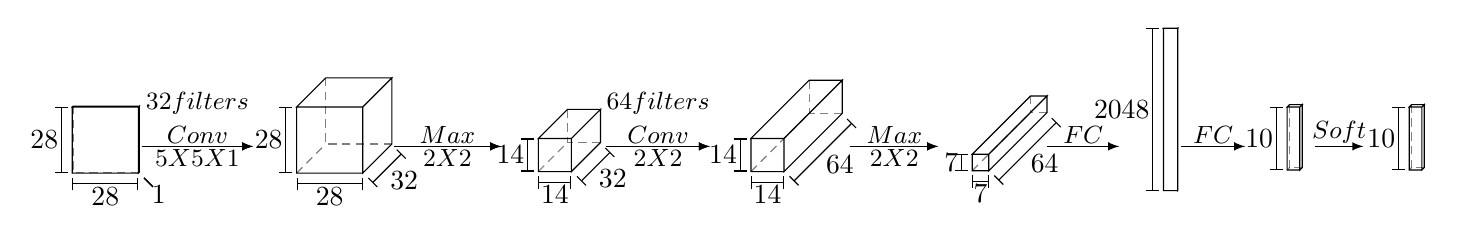
\begin{tikzpicture}[inner sep=1pt, >=latex, 
   label/.style={auto, inner sep=1pt, circle}
   ]
   
   \path (-10,-0.5) node (A) {$$}
   (-8.5,-0.5) node (B) {$$};
   \path (-6.8,-0.5) node (C) {$$}
   (-5.35,-0.5) node (D) {$$};
   \path (-4.1,-0.5) node (E) {$$}
   (-2.7,-0.5) node (F) {$$};
   \path (-1,-0.5) node (G) {$$}
   (0.2,-0.5) node (H) {$$};
   \path (1.5,-0.5) node (I) {$$}
   (2.5,-0.5) node (J) {$$};
   \path (3.2,-0.5) node (K) {$$}
   (4.1,-0.5) node (L) {$$};
   \path (4.9,-0.5) node (M) {$$}
   (5.6,-0.5) node (N) {$$};
   
   
   \draw[->] (A) -- node[anchor=north] {\small $5 X 5 X 1$} (B);
   \draw[->] (A) -- node[anchor=south, align=center] {\small $32 filters$ \\ \small $Conv$} (B);
   
   \draw[->] (C) -- node[anchor=north, align=center] {\small $2 X 2$} (D);
   \draw[->] (C) -- node[anchor=south] {\small $Max$} (D);
   
   \draw[->] (E) -- node[anchor=north, align=center] {\small $2 X 2$} (F);
   \draw[->] (E) -- node[anchor=south, align=center] {\small $64 filters$ \\ \small $Conv$} (F);
   
   \draw[->] (G) -- node[anchor=north, align=center] {\small $2 X 2$} (H);
   \draw[->] (G) -- node[anchor=south] {\small $Max$} (H);
   
   \draw[->] (I) -- node[anchor=south] {\small $FC$} (J);
   
   \draw[->] (K) -- node[anchor=south] {\small $FC$} (L);
   
   \draw[->] (M) -- node[anchor=south] {\small $Soft$} (N);
   
  \pic at (-10,0) {annotated cuboid={width=28, height=28, depth=1, scale = 0.03}};
  \pic at (-7.15,0) {annotated cuboid={width=28, height=28, depth=32, scale = 0.03}};
  \pic at (-4.5,-0.4) {annotated cuboid={width=14, height=14, depth=32, scale = 0.03}};
  \pic at (-1.8,-0.4) {annotated cuboid={width=14, height=14, depth=64, scale = 0.03}};
  \pic at(0.8,-0.6) {annotated cuboid={width=7, height=7, depth=64, scale = 0.03}};
  \pic at (3.2,1) {annotated rectangle={width=180, height=2048, depth=1, scale = 0.001}};
  \pic at (4.75,0) {annotated rectangle={width=2, height=10, depth=1, scale = 0.08}};
    \pic at (6.3,0) {annotated rectangle={width=2, height=10, depth=1, scale = 0.08}};
  
\end{tikzpicture}\
\end{figure*} 


$$\frac{\delta L_{y}}{\delta \theta}= 2*(f_w(x+g_{f,\theta} (x)) - r(f_w(x),t) * \frac{\delta f}{\delta\theta}$$

$$\frac{\delta f}{\delta \theta} = \frac{\delta f}{\delta g} * \frac{\delta g}{\delta \theta}$$ 



Parameters $\theta $ in each layer of the ATN are updated in every iteration like with standard gradient descent.\newline \newline
\noindent{{\bf 3.5 Experiments}\\
\indent We generated perturbed inputs from the non-MNIST dataset. Each image in 
the non-MNIST dataset is a 28x28 pixel image, giving a total of 
785 features in the input, including the bias. We first ran our 
experiments to break a simple 3 layer feed forward neural network. As mentioned above and seen in Figure 4, the input layer consists of 785 nodes. These 
are mapped onto the hidden layer that has 1000 nodes. The 1000 nodes of 
the hidden layer are then mapped to 10 nodes in the output layer, with 
each node representing the probability of the input corresponding to a 
particular class (classes are alphabets from 'A' to 'J'). Sigmoid 
activations were used in both the hidden, as well as the output layers. 
Upon training with 20,000 samples, this feed forward neural network had 
an error of 0.34 on the training set.

The ATN used to break the network described above was also a 3-layered 
feed forward neural network. As seen in Fig. 5, it has 785 nodes in the input layer, 1024 
nodes in the hidden layer and 784 nodes in the output layer. The 784 
nodes in the output layer each correspond to a perturbation to each of 
the 784 nodes in the input layer, without the bias term. We did not have 
any activations in the hidden layer and used $tanh$ activation in the 
output layer. As mentioned earlier, $tanh$ activations are used in the 
output layer to restrict the perturbations to be within the range of a 
neighbourhood, $\varepsilon $. We trained this model with a few 
different combinations for the choice of the reranking function between 
what was described above and a one hot encoding, and also the choice of 
using $L_{1}$ and $L_{2}$ for both $L_{x}$ and $L_{y}$. We 
were easily able to break this simple feed forward neural network, and 
increased the error rate to 0.9, regardless of the choice of target in each of these different combinations.


\section{Black Box Adversarial Transformative Networks}

In this section we extend our work to a targeted black box attack setting with Deep CNNs.\\

\noindent{{\bf 4.1 Target CNN}\\
 \indent As before, we define a target network as $ y = f_{w}(x) $ where $w$ is the parameter matrix of the network $f$, and $x$ is the input. Here $f$ is a Convolution Neural Network, having 2 convolution layers, 2 pooling layers and 2 fully connected layers. The input image is a 28 x 28 matrix which is convolved with 32 $5 x 5$ filters with same padding such that the output is same as the input(in size per activation map). Afterwards, we apply max-pooling with a $2 x 2$ kernel, with a stride of 2. This is followed by a second convolution layer with 64, $5 x 5$ filters using same padding as before, followed by another max-pooling operation with a $2 x 2$ kernel, with a stride of 2. It should be noted that the outputs after the convolution operation are passed through an activation function before the max-pooling operation. After this, the activations are flattened and passed to the first fully connected layer with 2048 hidden units, which is followed by passing the activations down to another fully connected layer with 10 nodes corresponding to the 10 character classes (A through J). This is then passed to softmax with 10 units to calculate the probabilities associated with each class. \\
 
 
 
 
 


\begin{figure*}[h!]
   \caption{Convolutional Adversarial Transformative Network}
   \label{fig:cclogo}
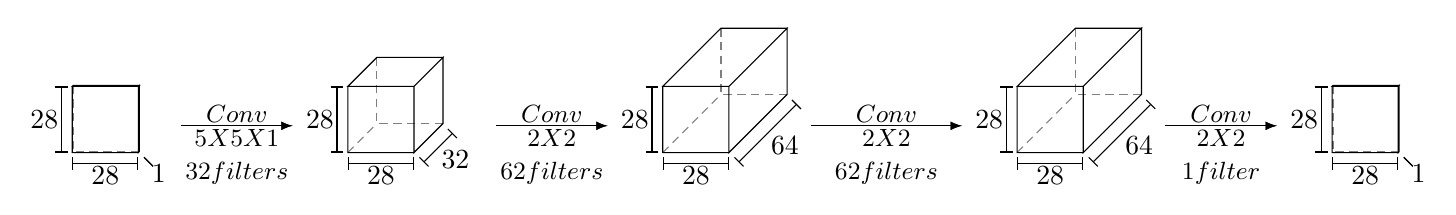
\begin{tikzpicture}[inner sep=1pt, >=latex, 
   label/.style={auto, inner sep=1pt, circle}
   ]
   
   \path (-9.5,-0.5) node (A) {$$}
   (-8,-0.5) node (B) {$$};
   \path (-5.5,-0.5) node (C) {$$}
   (-4,-0.5) node (D) {$$};
   \path (-1.5,-0.5) node (E) {$$}
   (0.5,-0.5) node (F) {$$};
   \path (3,-0.5) node (G) {$$}
   (4.5,-0.5) node (H) {$$};
   
   \draw[->] (A) -- node[anchor=north, align=center] {\small $5 X 5 X 1$ \\ \small $32 filters$} (B);
   \draw[->] (A) -- node[anchor=south] {\small $Conv$} (B);
   
   \draw[->] (C) -- node[anchor=north, align=center] {\small $2 X 2$ \\ \small $62 filters$} (D);
   \draw[->] (C) -- node[anchor=south] {\small $Conv$} (D);
   
   \draw[->] (E) -- node[anchor=north, align=center] {\small $2 X 2$ \\ \small $62 filters$} (F);
   \draw[->] (E) -- node[anchor=south] {\small $Conv$} (F);
   
   \draw[->] (G) -- node[anchor=north, align=center] {\small $2 X 2$ \\ \small$1 filter$} (H);
   \draw[->] (G) -- node[anchor=south] {\small $Conv$} (H);
   
  \pic at (-10,0) {annotated cuboid={width=28, height=28, depth=1, scale = 0.03}};
  \pic at (-6.5,0) {annotated cuboid={width=28, height=28, depth=32, scale = 0.03}};
  \pic at (-2.5,0) {annotated cuboid={width=28, height=28, depth=64, scale = 0.03}};
  \pic at (2,0) {annotated cuboid={width=28, height=28, depth=64, scale = 0.03}};
  \pic at (6,0) {annotated cuboid={width=28, height=28, depth=1, scale = 0.03}};
  
\end{tikzpicture}
\end{figure*} 
 
  \noindent{{\bf 4.2 Deep Convolutional ATN}\\
 \indent The ATN as defined before $$x' =  g_{f, \theta}(x)$$ is modified for the black box attack. Previously, we had access to the target Neural Network(f) parameters and we could compute the derivative of f with respect to g(ATN), but in black box attack these parameters are unknown and we need to modify the ATN definition to exclude this parameter. As such our new definition of ATN is $$x' =  g_{\theta}(x)$$. This represents an independent CNN where the number of input layer and output layer nodes are same, and we use it to find an encoding of the input image that is adversarial on the target image. The architecture of the Convolutional ATN is as follows: In total we have 4 convolutional layers. As before the size of input images is 28 x 28 which is convolved with 32, 3 x 3 filters. Note that we don't pass the output of the convolution layer through an activation function and we don't use subsampling either(since the output is an image and not a set of probabilities). This is followed by another convolution layer in which the outputs from previous convolution layer are convolved with 64, 3 x 3 filters. Usually after the traditional convolution layers, a traditional CNN will have a couple of fully connected layers. In this experiment, in order to mimic this architecture, we use 1 x 1 convolutions. This allows us to train the network faster and gives better results. We first convolve the outputs of the second convolution layer with 64, 1 x 1 filters, this is followed by convolution with 1, 1 x 1 filter. Note that the last convolution only uses 1 filter and after the convoltion we pass it through an activation function i.e tanh() function.\\
 
 \noindent{{\bf 4.3 Cost Function}\\
 \indent The cost function is modified from before to account for our black box setting as follows:
 
 $$\sum\limits_{x_{i}\in X}\beta L_{x}(g_{\theta}
(x_{i}), x_{i}) + L_{y}(f(g_{\theta}
(x_{i})),f(x))$$
 where $L_{x}$ as before is the difference between the generated adversarial example and the original input. Additionally, since this is a targeted attack, $L_{y}$ has to be tuned to nudge the Convolutional ATN towards learning a targeted adversarial example. As such $L_{y}$ is modified from the earlier version as follows:
 
 $$ L_{y} = L_{y}(f(g_{\theta}
(x_{i})),r(f(x), t)  $$

where r is the re-ranking function as described before. Intuitively $L_{x}$ represents the amount of distortion in the adversarial sample compared to the original sample and $L_{y}$ represents the difference between the output probabilities of the final layer for our adversarial example when passed through the target network and the output probabilities we want it to have biased towards the target class(say we want A classified as C).
 \newline

\noindent{{\bf4.4 Training}\\
To train the C-ATN, we first find the encoding of an input sample using the C-ATN which is the function $g()$, then we input this encoding into the target CNN which is the function $f()$. This gives the likelihood of how the target network classifies our encoding of the input sample. In this attack, the C-ATN only needs to be able to query the target network, no additional information of the target network is needed.

 We find the derivatives of the cost function with respect to $\theta$ and proceed with standard back propagation. Training can be done in batches or by samples individually. Computing the derivatives of $L_{x}$ is similar to what we did in the last section. For the $L_{y}$ part, we need to query the target CNN to get the value $f(g_{\theta}(x_{i}))$. Using these values, the re-ranking function determines based on a target class what values the target network should output for our adversarial sample. The difference between the two probability vectors is the loss. As an example, if a sample belongs to class 1, the target network will output probabilities close to the following vector: $f(x') = [ 1, 0, 0] $ (for a 3 class classification network). If we want the sample to be classified as a class 2 sample, the re-rank function will output something like this $r(f(x'), t) = [0, 1, 0]$. The difference of the two vectors is the loss which we need to minimize. Notice that this is one-hot encoding(just for demonstration), in practice we use actual probabilities. \newline

\noindent{{\bf 4.5 Experiments}\\
For the CNN, we used standard batch gradient descent with batch size $150$. In total our training set had 20,000 samples and in 2000 iterations we were able to get the training accuracy to about $99.4$ percent and our cross validation accuracy was about $93.5$ percent.\\
For the C-ATN part, we trained the network with a single sample each time. Everytime the sample moves through the network, the network creates an adversarial encoding of the sample, which is then used to query the original CNN which gives us what the target CNN thinks of this sample. Afterwards, we combine the loss as described before for both the distortion from the original sample, as well as the likelihood of the current sample being classified as the target adversarial sample and then back propagate on the C-ATN. Generally it took about 2000 iterations to generate each target adversarial sample.\\

\section{Results}
With the white box attack, we executed different combinations for $L_x$ and $L_y$ among $L_1$ and $L_2$. We also executed different re-ranking functions and compared our neighbourhood approach against the classical approach. Despite running all this against different targets we almost always obtained a high error rate of 0.9. In the black box setting, the targeted attack seems to work(for the most part) for another class than the target. For instance, a sample that was originally B and we set the target to be A, after finding the adversarial encoding of the sample, it was classified as H by the target CNN. The attack seems to work for a different target than the one intended. The attack works for the intended target sparingly.\\


\begin{figure}[h]
\includegraphics[scale=1.0]{pictures/original.png}
\includegraphics[scale=1.0]{pictures/class_as_D.png}
\includegraphics[scale=1.0]{pictures/class_as_A.png}
\includegraphics[scale=1.0]{pictures/class_as_I.png}
\includegraphics[scale=1.0]{pictures/class_as_H.png}
\includegraphics[scale=1.0]{pictures/class_as_C.png}
\includegraphics[scale=1.0]{pictures/class_as_G_and_D.png}
\includegraphics[scale=1.0]{pictures/evenly_distributed.png}



\caption{The left most image represents the original image, we set the C-ATN target as class A(i.e generate adversarial samples that are classified as A). The next image is the perturbed image that was classified as D by the target CNN, the image to its right was classified as A, the next image was classified as I, the image to its right was classified as H, the next image was classified as C, the following image to the right was classified as G and D with almost equal probabilities, and finally the last image above had probabilities equally distributed for more than 5 classes.  }
\end{figure} 

\begin{figure}[h]
\includegraphics[scale=1.0]{pictures/original_C.png}
\includegraphics[scale=1.0]{pictures/C_class_as_I.png}
\includegraphics[scale=1.0]{pictures/C_class_as_A.png}
\includegraphics[scale=1.0]{pictures/C_class_as_J.png}
\includegraphics[scale=1.0]{pictures/C_class_as_G.png}
\includegraphics[scale=1.0]{pictures/C_class_as_D.png}
\includegraphics[scale=1.0]{pictures/C_class_as_H_and_I.png}
\includegraphics[scale=1.0]{pictures/C_class_as_D_and_I.png}



\caption{The left most image represents the original image, we set the C-ATN target as class A(i.e generate adversarial samples that are classified as A). The next image is the perturbed image that was classified as I by the target CNN, the image to its right was classified as A, the next image was classified as J, the image to its right was classified as G, the next image was classified as D, the following image to the right was classified as H and I with almost equal probabilities, and finally the last image above was classified as D and I with almost equal probabilities.  }
\end{figure} 

\begin{figure}[h]
\includegraphics[scale=1.0]{pictures/first_original.png}
\includegraphics[scale=1.0]{pictures/A_class_as_H(2).png}
\includegraphics[scale=1.0]{pictures/A_class_as_B.png}
\includegraphics[scale=1.0]{pictures/A_class_as_D.png}
\includegraphics[scale=1.0]{pictures/A_class_as_J.png}
\includegraphics[scale=1.0]{pictures/A_class_A_and_I.png}
\includegraphics[scale=1.0]{pictures/A_class_as_D_and_I.png}
\includegraphics[scale=1.0]{pictures/A_class_as_A_D_H.png}




\caption{The left most image represents the original image, we set the C-ATN target as class B(i.e generate adversarial samples that are classified as B). The next image is the perturbed image that was classified as H by the target CNN, the image to its right was classified as B, the next image was classified as D, the image to its right was classified as J, the image to its right was classified as A and I with almost equal probabilities, the next image was classified as D and I with almost equal probabilities, the following image to the right was classified as A, D and H with almost equal probabilities.}
\end{figure} 
\section{Discussion}
The results of our experiments show that for simple ANNs, regardless of the choice of the cost function, re-ranking function or the activations used in the ATN, breaking the simple target ANN was not very difficult. This can be attributed to the lesser complexity of simple ANNs. This is not true for Deep Convolution Networks especially in the black box setting where the attacks work only infrequently. The C-ATN often generates advesarial samples for other targets than the one that is intended. Also, the choice of parameters matters in this case. For the cost function, $L_{x}$ is scaled down considerably and $L_{y}$ needs to be multiplied by a large number for the attack to succeed, this can be attributed to the lack of knowledge of the parameters of the target networks and inability to back propagate on the original network.
\section{Conclusion}
Many current methods of generating adversarial examples can be defended against. In our paper, we proposed two alternative attacks. The white box attack could access the internal parameters of the target network and yielded great results. The black box attack on the other hand did not perform as well, owing to the greater complexity of CNNs and not having access to the internal parameters of the target network. In conclusion, future work should focus on finding better cost functions for black box attacks.
\section{Source Code}
The source code of the project can be found at the following url\\
{\itshape https://github.com/Zainul-Abi-Din/DeepLearning}










\bibliographystyle{abbrv}
\begin{thebibliography}{10}


\bibitem{1}
S.~M. Moosavi-Dezfooli, A.~Fawzi, P.~Frossard
\newblock DeepFool: a simple and accurate method to fool deep neural networks.
\newblock In {\em IEEE Conference on Computer Vision and Pattern Recognition (CVPR)}, 2016. \newline


\bibitem{2}
S. ~Alfeld, X. ~Zhu, and P. ~Barford
\newblock Data poisoning attacks against
autoregressive models.
\newblock In {\em Thirtieth AAAI Conference on Artificial
Intelligence}, 2016. \newline

\bibitem{3}
K. ~Grosse, N.~Papernot, P.~Manoharan, M.~Backes, and P.~McDaniel
\newblock Adversarial perturbations against deep neural networks for malware
classification
\newblock In {\em Thirtieth AAAI Conference on Artificial
Intelligence}, 2016. \newline


\bibitem{4}
Szegedy, Christian, Zaremba, Wojciech, Sutskever, Ilya, Bruna, Joan, Erhan, Dumitru, Goodfellow, Ian J., and Fergus, Rob.
\newblock  Intriguing properties of neural networks.
\newblock In {\em ICLR, abs/1312.6199, 2014b}, 2014. URL http: //arxiv.org/abs/1312.6199. \newline

\bibitem{5} 
Ian J. Goodfellow, Jonathan Shlens and Christian Szegedy
\newblock Explaining and Harnessing Adversarial Examples
\newblock In {\em ICLR}, 2015. \newline

\bibitem{6} 
Jia Deng, Wei Dong, Richard Socher, Li-Jia Li, Kai Li and Li Fei-Fei
\newblock ImageNet: A Large-Scale Hierarchical Image Database
\newblock In {\em CVPR}, 2009. \newline

\bibitem{7} 
Papernot, N., McDaniel, P., Jha S., Fredrikson, M., Celik, Z. B., And Swami, A.
\newblock The limitations of deep learning in adversarial settings. 
\newblock In {\em IEEE}, 2016. \newline

\bibitem{8}
Nicholas Carlini David Wagner
\newblock Towards Evaluating the Robustness of Neural Networks
\newblock In {\em arXiv
preprint arXiv:1608.04644}, 2016. \newline

\bibitem{9}
Nicolas Papernot, Patrick McDaniel, Somesh Jha, Matt Fredrikson, Z. Berkay Celik, Ananthram Swami
\newblock The Limitations of Deep Learning
in Adversarial Settings
\newblock In {\em	arXiv:1511.07528}, 2015. \newline

\bibitem{10}
Pin-Yu Chen, Huan Zhang, Yash Sharma, Jinfeng Yi, Cho-Jui Hsieh
\newblock ZOO: Zeroth Order Optimization based Black-box Attacks to Deep Neural Networks without Training Substitute Models
\newblock In {\em		arXiv:1708.03999}, 2017. \newline

\bibitem{11}
Nicholas Carlini and David Wagner.
\newblock . Adversarial Examples Are Not Easily
Detected: Bypassing Ten Detection Methods. 
\newblock In {\em	 arXiv:1705.07263}, 2017. \newline

\bibitem{12}
Aleksander Madry, Aleksandar Makelov, Ludwig Schmidt, Dimitris Tsipras, and
Adrian Vladu
\newblock Towards Deep Learning Models Resistant to Adversarial
Attacks.
\newblock In {\em	 arXiv:1706.06083}, 2017. \newline

\bibitem{13}
Shumeet Baluja and Ian Fischer
\newblock Adversarial Transformation Networks:
Learning to Generate Adversarial Examples
\newblock In {\em	arXiv:1703.09387v1}, 2017. \newline

\bibitem{14}
Nicolas Papernot, Patrick McDaniel, Somesh Jha, Matt Fredrikson, Z. Berkay Celik, Ananthram Swami
\newblock Adversarial The Limitations of Deep Learning in Adversarial Settings
\newblock In {\em 	arXiv:1511.07528}, 2015. \newline


\end{thebibliography}

\end{document}  % This is where a 'short' article might terminate
